\documentclass[titlepage,twoside,10pt,twocolumn,a4paper]{article}
\usepackage{abstract_style_2018}

\newcommand{\gc}{ {\rm g} }
\newcommand{\er}{ {\rm e} }
\newcommand{\bra}[1]{\langle{#1}|}
\newcommand{\ket}[1]{|{#1}\rangle}
\newcommand{\s}[1]{ \hat{\sigma}_{#1}}
\newcommand{\dg}{^\dagger}
\newcommand{\erf}[1]{Eq.~(\ref{#1})}
\newcommand{\tr}[1]{{\rm Tr}\sq{ {#1} }}
\newcommand{\sq}[1]{\left[{#1}\right]}
\newcommand{\frf}[1]{Fig.~\ref{#1}}

% due to .pdf image inclusion, compile eg. with
% pdflatex appc-aip-template-latex

\begin{document}

\titleblock{

\papertitle{Quantum master equations for entangled qubit environments}

\authors{\underline{Shakib Daryanoosh}$^{1*}$, Ben Q. Baragiola$^{2,1}$, Tom Guff$^1$ and Alexei Gilchrist$^{1}$}

$^1$\affiliation{Centre for Engineered Quantum Systems, Department of Physics and Astronomy, Macquarie University, Sydney, NSW 2122, Australia}
$^2$\affiliation{Centre for Quantum Computation and Communication Technology, School of Science, RMIT University, Melbourne, Victoria 3001, Australia}
$^*$\contact{shakib.daryanoosh@mq.edu.au}
}

\starttext
\emph{
In this work we study Markovian dynamics of $N$ independent quantum systems where each is subject to a corresponding irreversible environmental channel. 
Using the framework of repeated quantum interactions, we derive master equations (MEs). In particular, we thoroughly investigate the evolution of the system for two-qubit baths. It is shown that (1) the presence of antidiagonal coherences in the environment's state (in the local energy basis) is a necessary condition for entangling two remote systems, and (2) for maximally entangled two-qubit baths the joint system does not have a unique steady state.} %We further derive a master equation for the general case of $N$-qubit environments. %It is proved that, in the weak coupling regime, maximally $N$-qubit entangled baths do not lead to correlating all the subsystems.


%\section{Introduction}
Inherent properties of quantum physics such as entanglement and coherent superposition play an important role in the revolution promised by quantum technologies. However, quantum systems tend to lose these key characteristics due to interacting with the outside world they coupled to. Therefore, a challenging task is to maintain these properties over a longer period by engineering the environments \cite{MulLin12} and the form of system-environment interactions. 

One approach to study such open quantum systems is that of repeated quantum interactions \cite{Pel10, LorPal17}. In this formalism the environment is comprised of a chain of identical and independent quantum systems which couple to the system one by one and are then traced out. %Thus, the environment does not retain any memory, and as a result the Markovian approximation can be employed. 
In the continuous limit this leads to the construction of a ME. This formalism has been employed in the context of quantum thermodynamics \cite{StrEsp17} and quantum optics and information \cite{GroCom17}. In the following we present some results for preparing the environment in entangled two-qubit states. 

%\section{Results} 
Let us consider the case in which the two subsystems are identical two-level atoms (qubits) resonantly interacting with a pure Bell state environment, say $\ket{\psi_E} = \ket{\Phi^+} =( \ket{\er\er} + \ket{\gc\gc} )/{\sqrt{2}}$, via the interaction Hamiltonian $\hat{H}_I = \sum_{l=1}^2 \lambda_l \big( \hat \sigma_{l}^\dagger \otimes \hat\sigma_{l} + {\rm H. c.}\big)$. Here $\hat\sigma_{l}$ refers to the lowering operator for the $l$-th qubit in the system and environment, respectively, and $\lambda_l$ is the coupling strength between the $l$-{th} atom and its qubit. One can then construct the appropriate ME for the reduced state matrix $\hat{\rho}$ of the joint system by expanding the unitary time evolution $U_I = e^{-i\hat H_I \Delta t}$ up to the second order in the small interaction time interval $\Delta t$ and taking the continuous limit of the dynamical map $\hat \rho_0 \rightarrow {\rm Tr}_E [\hat{U}_I \hat \rho_0 \otimes \hat \rho_E \,\hat{U}_I^\dagger]$, where $\rho_0$ is the initial state of the composite system and $\hat{\rho}_E = \ket{\psi_E}\bra{\psi_E}$, to obtain \cite{DarGil18}
\begin{align}  \label{ME:Bell:phi}
	\dot{\hat{\rho}}(t) =&  \frac{\gamma}{2} ( \mathcal{D} [\hat{L}] +  \mathcal{D} [\hat{L}^\dagger])\hat{\rho}.
\end{align}
Here the Lindblad operator is $\hat{L} = \s{1} + \s{2}^\dagger$, the coupling strengths are taken to be equal $\gamma = \lambda^2 \Delta t$, and ${\cal D}[\hat o] \hat{\rho} = \hat o \rho \hat o\dg - \left\{\hat o\dg \hat o, \hat\rho\right\}_+/2$. It turns our that if the bath is prepared {\it exactly} in $\ket{\Phi^+}$ then the system's steady state (limit of $t \rightarrow \infty$) and its amount of non-classical correlations depends on its initial state. This is shown in \frf{fig:LN} (dashed-green) by using logarithmic negativity $LN(\hat{\rho}) := {\rm log}_2 ([\sqrt{\hat{\varrho}\dg \hat{\varrho}}])$ to quantify entanglement, where $\varrho$ is the partial transpose of $\rho$. The initial state varies according to $\ket{\psi_0(\theta)} = \sin \theta \ket{\Phi^+} + \cos \theta \ket{\Phi^-}$. It can be clearly seen that the initial entanglement in the system (solid-grey curve) is preserved for $\theta \in [0,\pi/4)$ and it is completely destroyed for $(\pi/4, \pi/2]$. Note that at $\theta=\pi/4$ the system is in the product state $\ket{\er\er}$. As a result this protocol never creates entanglement. However, when the environment is in a non-maximally entangled state, the ME has a unique entangled steady state. For example, consider $\ket{\Phi^+(\epsilon)} = (\ket{\er\er} + \sqrt{1+\epsilon} \ket{\gc\gc}) / \sqrt{2+\epsilon}$ for $0 < \epsilon \ll 1$ which is very close to the Bell-state. Then the steady state of the system is highly entalged $LN(\hat\rho) \approx 1$ independent of the initial state, see \frf{fig:LN} (dotted-blue line). The above argument also holds for other Bell-state baths. It can be shown that preparing the bath in $\ket{\Phi^+(\epsilon)}$ drives the system to a two-mode squeezed state for the case of two remote optical cavities, and deriving of a master equation for the general case of $N$-qubit environments is also straightforward \cite{DarGil18}.

%
\begin{figure}[ht!]
\centerline{
  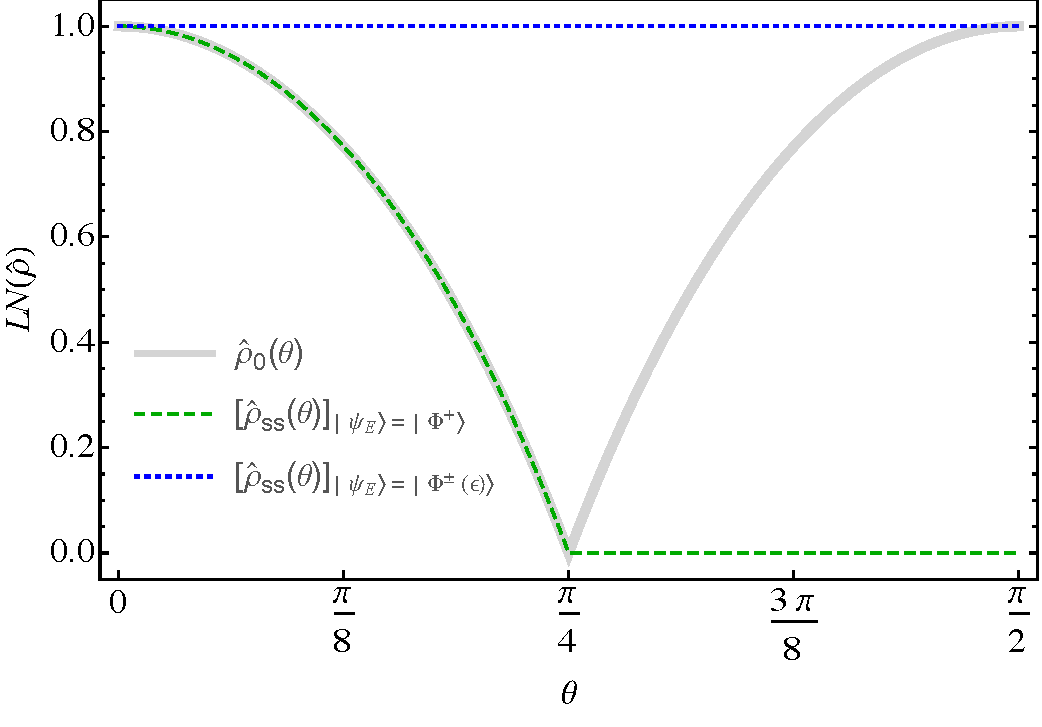
\includegraphics[width=\columnwidth]{fig.pdf}
} 
\caption{Entanglement of the atomic state. }
\label{fig:LN}
\end{figure}
%when the two-qubit bath is prepared in the $\ket{\Phi^+_E}$ Bell state. The initial two-atom state $\hat{\rho}_0(\theta)$ is parameterized by $\theta$, \erf{phi:plus:minus}. We also include plots for non-maximally entangled atomic states, $\ket{\Phi^\pm(\epsilon)}$, that deviate from Bell states by $\epsilon = 0.001$, \erf{eq:nearBell}.  (a) Entanglement as quantified by the logarithmic negativity, \erf{log:neg}, for which $LN(\hat{\rho}) \approx 1$. (b) State purity, $\tr{\hat{\rho}^2}$. Note that for $\theta<\theta_c = \pi/4$, the gray curve and dashed blue curve exactly coincide. That is, initial entanglement is preserved despite the fact that the state becomes mixed. Beyond $\theta_c$ the steady state is no longer entangled, and the minimum purity, 0.25, occurs at $\theta = \pi/3$

\begin{thebibliography}{2}

\bibitem{MulLin12}
{M. M{\"u}ller, {et al.,}``Engineered Open Systems and Quantum Simulations with Atoms and Ions,'' in Advances In Atomic, Molecular, and Optical Physics, vol. 61. Academic Press, 2012, pp. 1}

\bibitem{Pel10}
{C. Pellegrini,  Ann. Inst. H. Poincar\'e Probab. Statist. vol. 46, pp. 924, (2010)}

\bibitem{LorPal17}
{S. Lorenzo, F. Ciccarello, and G. Massimo Palma, Phys. Rev. A vol. 96, pp. 032107, (2017)}

\bibitem{StrEsp17}
{P. Strasberg, G. Schaller, T. Brandes, and M. Esposito, Phys. Rev. X vol. 7, pp. 021003, (2017)}

\bibitem{GroCom17}
{J. A. Gross, C. M. Caves, G. J. Milburn, and J. Combes,  Quantum Sci. Technol. vol. 3, pp. 024005, (2017)}

\bibitem{DarGil18}
{S. Daryanoosh, B. Q. Baragiola, T. Guff, and A. Gilchrist,  arXiv, (2018)}

%\bibitem{MulLin12}
%{M. M{\"u}ller, {et al.,}``Engineered Open Systems and Quantum Simulations with Atoms and Ions,'' in Advances In Atomic, Molecular, and Optical Physics, vol. 61. Academic Press, 2012, pp. 1}
%
%\bibitem{Pel10}
%{C. Pellegrini, ``Markov chains approximation of jump-diffusion stochastic master equations,"  Ann. Inst. H. Poincar\'e Probab. Statist. vol. 46, pp. 924, (2010)}
%
%\bibitem{LorPal17}
%{S. Lorenzo, F. Ciccarello, and G. Massimo Palma, ``Markov chains approximation of jump-diffusion stochastic master equations,"  Phys. Rev. A vol. 96, pp. 032107, (2017)}
%
%\bibitem{StrEsp17}
%{P. Strasberg, G. Schaller, T. Brandes, and M. Esposito, ``Quantum and Information Thermodynamics: A Unifying Framework Based on Repeated Interactions,"  Phys. Rev. X vol. 7, pp. 021003, (2017)}
%
%\bibitem{GroCom17}
%{J. A. Gross, C. M. Caves, G. J. Milburn, and J. Combes, ``Qubit models of weak continuous measurements: markovian conditional and open-system dynamics,"  Quantum Sci. Technol. vol. 3, pp. 024005, (2017)}
%
%\bibitem{DarGil18}
%{S. Daryanoosh, B. Q. Baragiola, T. Guff, and A. Gilchrist ``Quantum master equations for entangled qubit environments,"  arXiv, (2018)}

\end{thebibliography}

\end{document}

%Copy this template and the file \texttt{abstract\_style\_2018.sty} in the same
%folder. Please do not change the style file, it contains all the page
%settings and the commands.
%
%\section{Conclusion}
%Use \verb|\titleblock{}|, \verb|\papertitle{}|, \verb|\authors{}|,
%\verb|\affiliation{}| and \verb|\contact{}| to define the title,
%authors, affiliations and correspondance email adress.  The presenting
%author is indicated by an asterix * and their email address should be
%given below the affiliations. Affiliations should be indicated by
%numbers.

%\section{Main text}
%Your main text should be added after the \verb|\starttext| command.
%Equations can be added and referenced as usual in \LaTeX{}. For example,
%Eq.(\ref{eqn:schrodinger}) below
%%
%\begin{equation}
%i \hbar \frac{\partial \psi}{\partial t}=H \psi,
%\label{eqn:schrodinger}
%\end{equation}
%%
%You may also want to add figures to your abstract. This can be done using the command:
%%
%Figures should be captioned. If you have multiple figures we suggest
%that you present them as subfigures in a single image file and name
%them Fig.1a, Fig.1b, etc. In this way you save space for your text.
%
%
%\section{Format of References}
%Citations are also added in the standard \LaTeX{} manner using
%\verb|\cite{ref_label}|. When citing at the beginning of a senctence,
%write ``Reference \verb|\cite{texref}| ...''.  For a reference with
%six or more authors, “et al.” may be used. In other cases, list all
%authors. Capitalize only the first word in a paper title, except for
%proper nouns and element symbols. Even if they have been submitted for
%publication, unpublished papers should be cited as “unpublished”
%\cite{unpublished}. Papers that have been accepted for publication
%should be cited as “in press” \cite{inpress}.
%
%\section{Format and submission steps}
%\begin{itemize}
%   \itemsep0em
%\item The page layout is defined in the \texttt{abstract\_style\_2018.sty} style file. {\bf Don't change it}.
%\item  Generate a \texttt{pdf} file. Make sure that your pdf document \textbf{matches the length requires for your conference (AIP/AOS/ACOFT/COMMAD)}.
%\item Submit the \texttt{.pdf} file to the abstract submission via \href{www.aip2018.org.au}{www.aip2018.org.au}.
%\end{itemize}


